\documentclass[a4paper,12pt]{article}
%-----------
\usepackage{lipsum}
\usepackage{amssymb}
\usepackage{amsmath}
\usepackage{graphicx}
\usepackage{placeins}
\usepackage{a4wide}
\usepackage[dutch]{babel}
\usepackage{multicol}
\usepackage[makeroom]{cancel}
\usepackage{enumerate}
\usepackage{epstopdf}
\usepackage{lscape}
%\usepackage{caption}
\usepackage[labelfont=bf]{caption}
\usepackage{hyperref}
%-----------
\usepackage[utf8]{inputenc}
\usepackage[T1]{fontenc}
%-----------
\title{Inleiding Programmeren: \\ Verwerking Examenopdracht}
\date{20-05-2019}
\author{Stoops Tom \\ 2 Ba Fysica}
%-----------
\newcommand{\paf}[2]{\frac{\partial #1}{\partial #2}}
%syntax: \partaf{A}{x} is partiele afgeleide van A naar x geevalueerd in x
\newcommand{\prop}[2]{s_{#2}^2\cdot\left(\paf{#1}{#2}\right)^2}
%syntax: analoog aan partaf, maar dan voor de propagatieformule (enkel sommeren erover en onder een wortel plaatsen: s_x = \sqrt{\prop{A}{a}+\prop{B}{b}+\ldots}
\renewcommand{\thefootnote}{\Roman{footnote}}
%\renewcommand{\phi}{\varphi}
\newcommand{\af}[3]{\frac{d^{#1}#2}{d {#3}^{#1}}}
%syntax: \af{4}{y}{x} is de 4de afgeleide van y naar x, voor 1ste afgeleide de eerste {} gewoon leeg laten!
\newcommand{\ste}{$^\mathrm{ste}\ $}
\newcommand{\de}{$^\mathrm{de}\ $}
%syntax: gewoon achter getal plaatsen
\newcommand{\p}[1]{\left(#1\right)}
\newcommand{\s}[1]{\left[#1\right]}
\newcommand{\avg}[1]{\left\langle#1\right\rangle}
\newcommand{\ta}{$\pm$}
\newcommand{\cirkel}[1]{\raisebox{.5pt}{\textcircled{\raisebox{-1.1pt} {#1}}}}
\let\oldarctan\arctan
\renewcommand{\arctan}[1]{\oldarctan\p{#1}}
%-----------
\captionsetup{width=0.8\textwidth}
%-----------
\begin{document}
\pagenumbering{arabic}
\maketitle
\tableofcontents

\newpage
\section{Inleiding}
  \noindent
  ...

\newpage
\section{Problemen}
  \subsection{Probleem 1: Superpositie van source-sink pair}
    \noindent
    Voor de eerste opdracht bekeken we de superpositie van een source-sink paar. Voor de configuratie waar de source geplaatst is op $\p{-1,0}$ en sink op $\p{1,0}$ beide met gelijke sterkte $Q$ vinden we de stroomlijnen en snelheidsvectoren zoals weergegeven op figuur \ref{probleem1_1}, wat een zeer intu\"itief resultaat is. Op figuur \ref{probleem1_2} zijn de equipotentiaallijnen weergegeven op een contourplot. Dit komt ook overeen met intu\"itie, op figuur \ref{probleem1_3} zijn de plots samen weergegeven. Op deze figuur kan men duidelijk de relatie tussen snelheidsvectoren en potentiaal vinden zoals gegeven in \cite{opdracht}:

    \begin{equation*}
      \overline{v}\p{x,y} = \overline{\nabla\phi}\p{x,y}
    \end{equation*}

    \noindent
    Waar de snelheidsvector $\overline{v}\p{x,y}$ gegeven is door de gradi\"ent van het potentiaalveld $\phi\p{x,y}$. Dit is ook duidelijk uit de figuur, daar de gradi\"ent het pad van sterkste stijging geeft en dus loodrecht staat op de krommen van gelijke waarde.\\

    \noindent
    Vervolgens is het ook nog interessant om te bekijken wat er gebeurt indien de source en sink verschillende sterktes hebben: $Q_{source} \neq Q_{sink}$, in figuur \ref{probleem1_4} is dit gegeven voor een source die een factor 4 sterker is dan de sink. Ook hier is het resultaat vrij intu\"itief; de source is opmerkelijk sterker dan de sink, waardoor er een deel van de stroomlijnen die vanuit de source vertrekken in de sink terecht komen, maar ook een deel die gewoon aan de sink voorbijlopen.\\

    \noindent
    Tot slot voor deze opdracht bestudeerden we ook nog wat er gebeurde indien de sterktes van de source en sink afhankelijk werden van de afstand tot elkaar:

    \begin{equation*}
      Q\cdot\ell = c^{te} \quad\text{met } Q = Q_{source} = Q_{sink}
    \end{equation*}

    \noindent
    Waar $\ell$ de afstand tussen de source en sink is. We op de verschillende plots van figuur \ref{probleem1_5} dat voor de limiet waar $\ell\rightarrow0$ dat het patroon van stroomlijnen convergeert naar dat van een source-sink doublet zoals gegeven in de opdracht \cite{opdracht}.\\

    \paragraph{Opmerking:} In de code (bijgeleverd in \texttt{.cpp}-formaat) werd er voor source en sink slechts \'e\'en klasse ge\"implementeerd daar we een sink kunnen interpreteren als een source met negatieve sterkte.

    \FloatBarrier
    \begin{figure}[ht!]
      \centering
      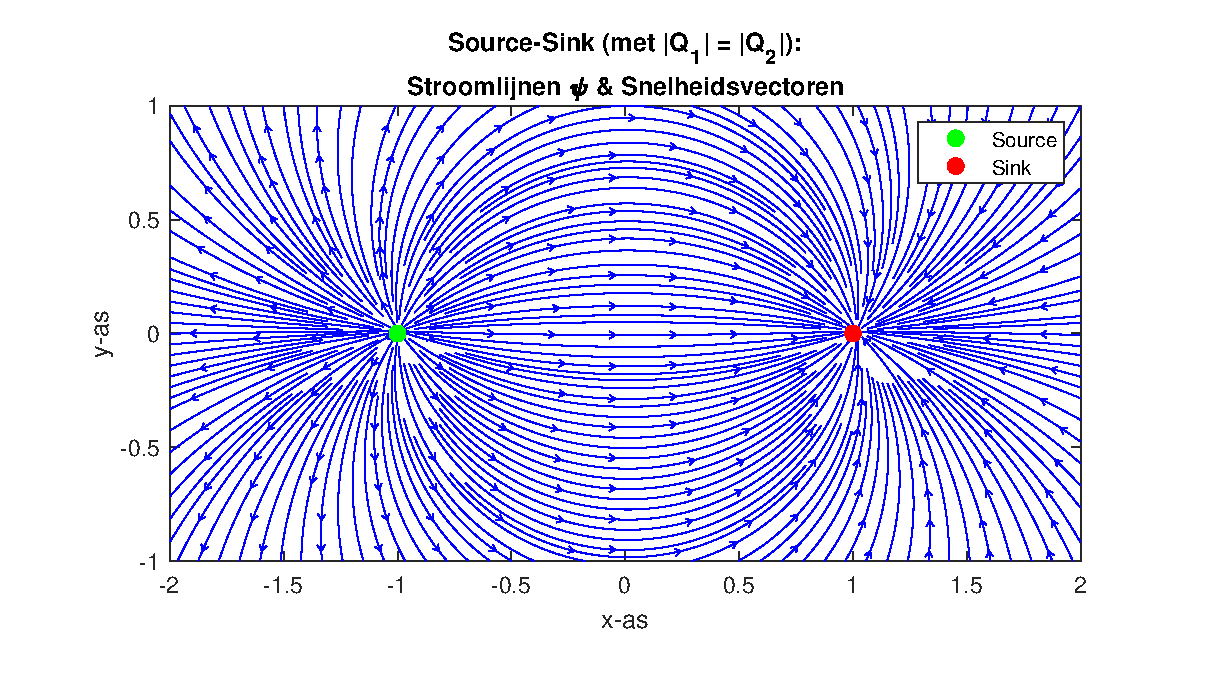
\includegraphics[width = \textwidth]{plots/probleem1_1.eps}
      \caption{Weergave van de stroomlijnen en snelheidsvectoren voor een source-sink paar.}
      \label{probleem1_1}
    \end{figure}
    \begin{figure}[ht!]
      \centering
      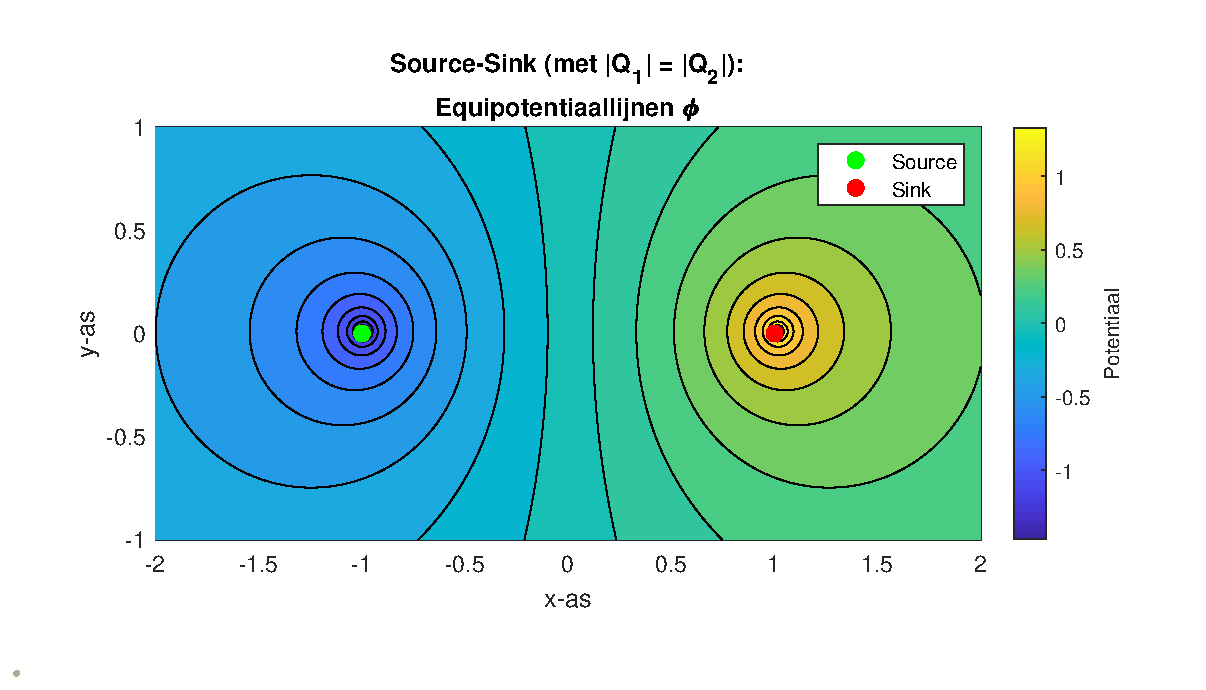
\includegraphics[width = \textwidth]{plots/probleem1_2.eps}
      \caption{Weergave van equipotentiaallijnen voor een source-sink paar.}
      \label{probleem1_2}
    \end{figure}
    \begin{figure}[ht!]
      \centering
      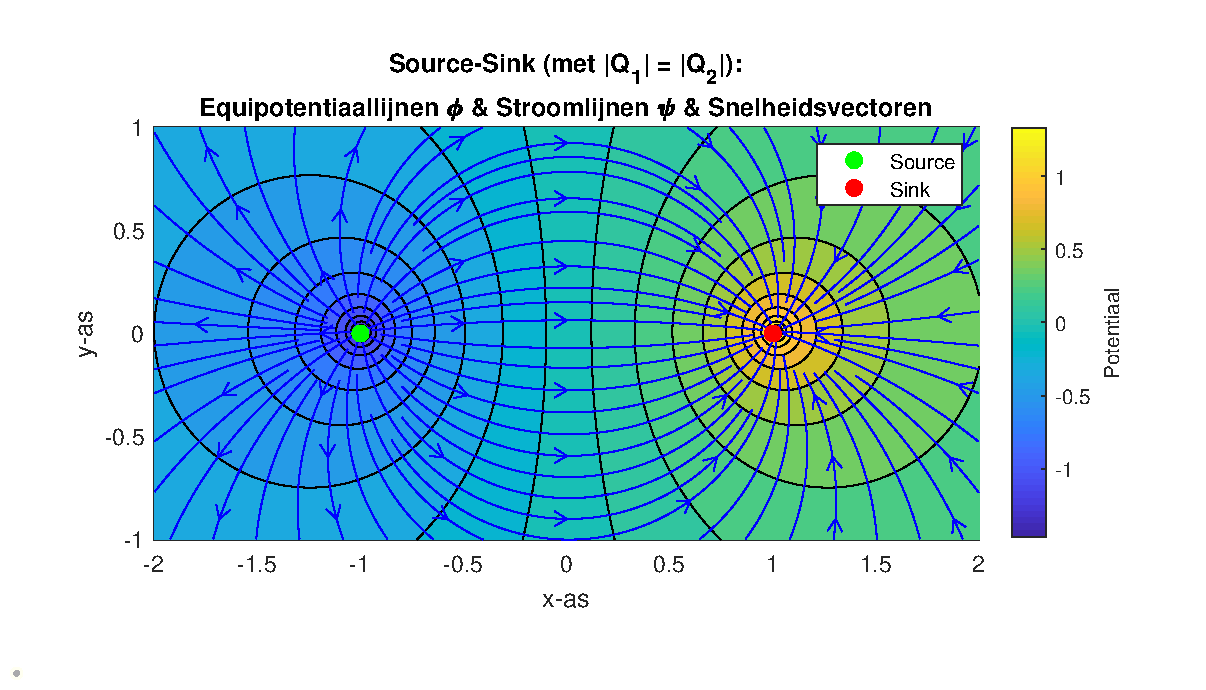
\includegraphics[width = \textwidth]{plots/probleem1_3.eps}
      \caption{Weergave van stroomlijnen, snelheidsvectoren, en equipotentiaallijnen voor een source-sink paar.}
      \label{probleem1_3}
    \end{figure}
    \begin{figure}[ht!]
      \centering
      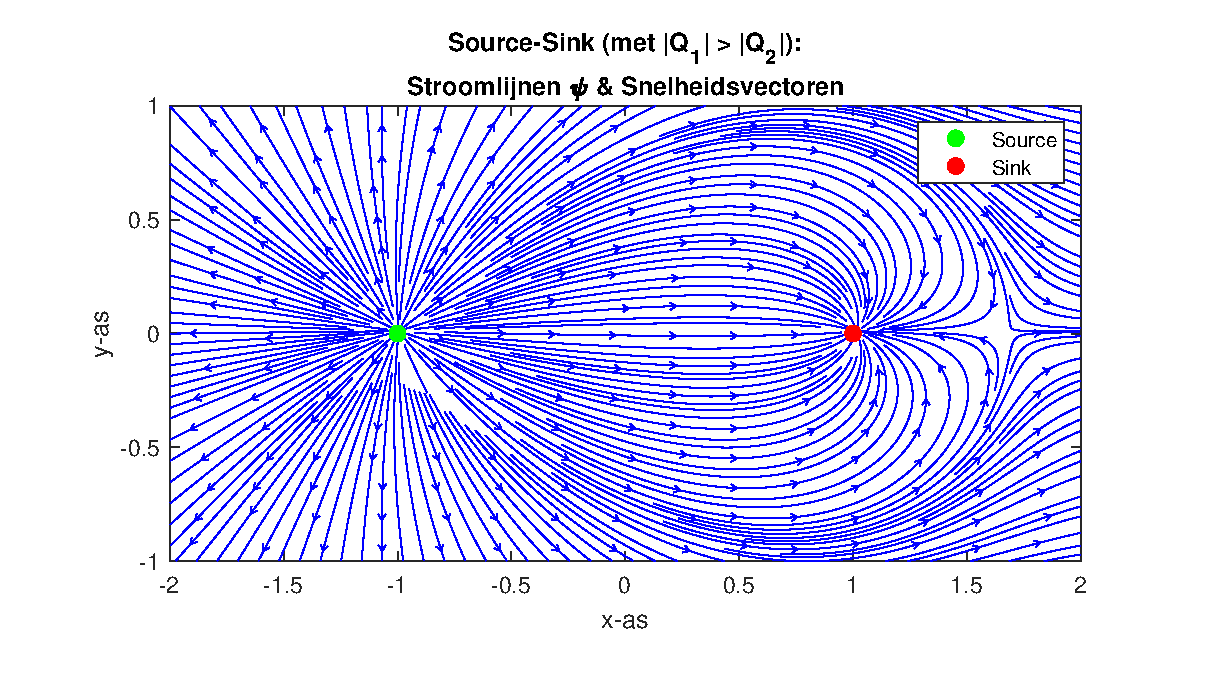
\includegraphics[width = \textwidth]{plots/probleem1_4.eps}
      \caption{Weergave van stroomlijnen en snelheidsvectoren voor een source-sink paar waarbij de source een factor 4 keer sterker is dan de sink.}
      \label{probleem1_4}
    \end{figure}
    \begin{figure}[ht!]
      \centering\vspace{-1.5cm}
      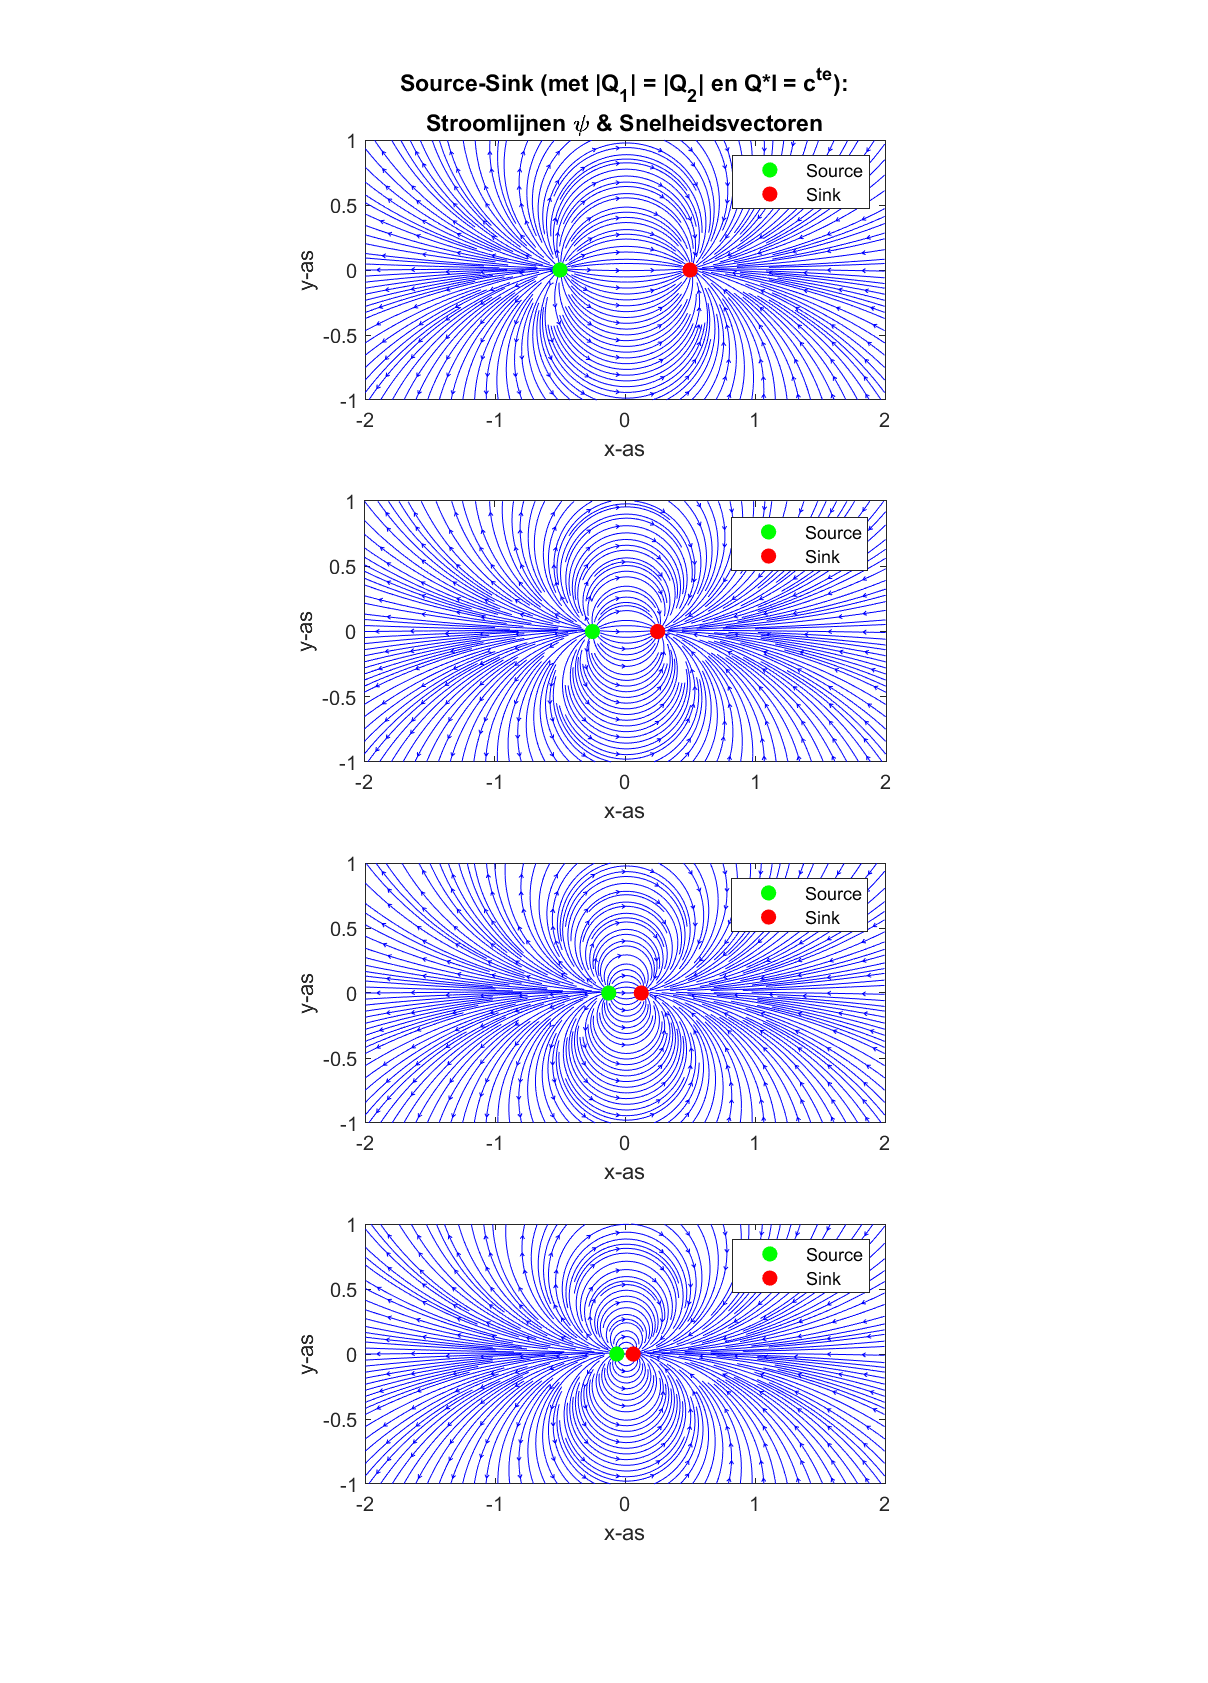
\includegraphics[width = \textwidth]{plots/probleem1_5.eps}\vspace{-1cm}
      \caption{Source-sink paar waarbij men observeert dat voor de limiet van $\ell\rightarrow0$ men een source-sink doublet bekomt, daar $Q\cdot\ell=c^{te}$.}
      \label{probleem1_5}
    \end{figure}
    \FloatBarrier

  \newpage
  \subsection{Probleem 2: Een source in uniforme stroming}
    \noindent
    In deze opdracht werden de stroomlijnen en snelheidsvectoren gevisualiseerd voor een source in een uniforme stroom. We zien op figuur \ref{probleem2_1} een vrij intu\"itief resultaat waar de uniforme stroom afgebogen wordt in de buurt van de source en daar de stroom van de source botst op de uniforme stroom vinden we een stagnatiepunt. Dit stagnatiepunt wordt gekenmerkt door $\left|\overline{v}\p{x_{stagnatie},y_{stagnatie}}\right| = 0$. We kunnen eenvoudig de formule afleiden om de positie van dit stagnatiepunt te bepalen.\\

    \noindent
    Allereerst merken we op dat het probleem translatie-invariant is langs de $y$-as voor het geval van een uniforme stroming langs de $x$-as. Er volgt dus direct dat:

    \begin{equation*}
      y_{stagnatie} = y_{source}
    \end{equation*}

    \noindent
    Dan kunnen we voor de $x$-positie van het stagnatiepunt gebruik maken van het principe van superpositie, waaruit volgt dat:

    \begin{equation*}
      \overline{v}_{totaal} = \overline{v}_{uniform} + \overline{v}_{source}
    \end{equation*}

    \noindent
    We kunnen deze vergelijking dan nog splitsen per component, gezien we al weten waar de $y$-component van het stagnatiepunt zal zijn, beschouwen we enkel de $x$-component van de vector:

    \begin{equation*}
      v_{totaal,x} = v_{uniform,x} + v_{source,x}
    \end{equation*}

    \noindent
    Uit de opdracht \cite{opdracht} weten we ook dat:

    \begin{equation*}
      \left\{
      \begin{align}
        v_{uniform,x}\p{x,y} &= U_\infty\cos\alpha \\
        v_{source,x}\p{x,y}  &= \frac{Q}{2\pi}\frac{\p{x-x_{source}}}{\p{x-x_{source}}^2+\p{y-y_{source}}^2}
      \end{align}
      \right.
    \end{equation*}

    \noindent
    Invullen dat $\alpha=0$ en optellen om $v_{totaal,x}$ te verkrijgen levert:

    \begin{equation*}
      v_{totaal,x} = U_\infty+\frac{Q}{2\pi}\frac{\p{x-x_{source}}}{\p{x-x_{source}}^2+\p{y-y_{source}}^2}
    \end{equation*}

    \noindent
    We zoeken $\p{x_{stagnatie}, y_{stagnatie}}$ opdat $v_{totaal,x} = 0$, we vullen alvast voor de $y$-waarde in dat $y = y_{stagnatie} = y_{source}$, waardoor de uitdrukking vereenvoudigt tot:

    \begin{equation*}
      0 = U_\infty+\frac{Q}{2\pi}\frac{1}{x_{stagnatie}-x_{source}}
    \end{equation*}

    \noindent
    Herschikken levert dan eenvoudigweg:

    \begin{equation*}
      x_{stagnatie} = x_{source}-\frac{Q}{2\pi U_\infty}
    \end{equation*}

  \newpage
    \noindent
    Er volgt dus dat het stagnatiepunt gelegen is op de co\"ordinaat:

    \begin{equation*}
      \p{x,y} = \p{x_{source}-\frac{Q}{2\pi U_\infty}, y_{source}}
    \end{equation*}

    \noindent
    Dit kan ook met de simulatie aangetoond worden daar we op het contourplot weergegeven op figuur \ref{probleem2_2} zien dat op deze co\"ordinaat de norm van de snelheidsvector nul wordt. \\

    \noindent
    Tot slot van deze opdracht zien we ook nog op figuur \ref{probleem2_1} dat er een verdelende stroomlijn zichtbaar is langs de $x$-as voor $x\in]-\infty,x_{stagnatie}]$. Alle stroomlijnen boven deze lijn zullen langs boven over de source lopen, alle stroomlijnen hieronder zullen onder de source lopen. De halve ovaal waar de stroomlijnen van de uniforme stroom en de source elkaar ontmoeten noemt met de Rankine half body

    \FloatBarrier
    \begin{figure}[ht!]
      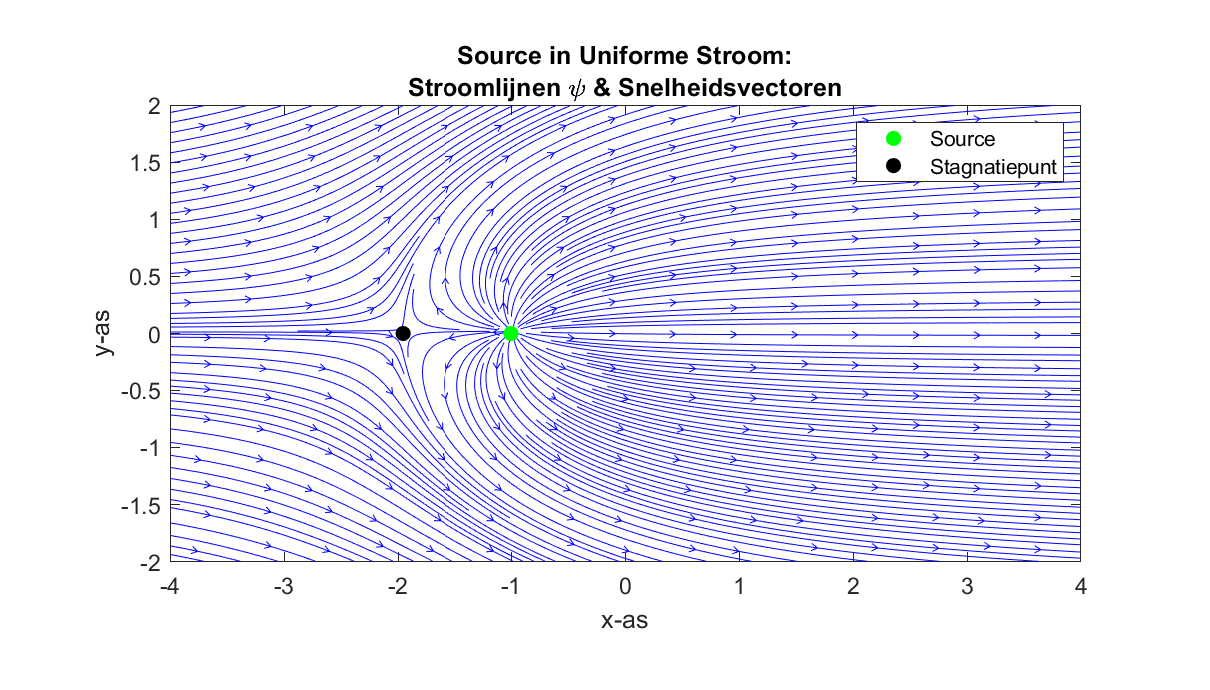
\includegraphics[width = \textwidth]{plots/probleem2_1.eps}
      \caption{Een source in uniforme stroming met stagnatiepunt en verdelende stroomlijn lopende langs de $x$-as in het domein $]-\infty,x_{stagnatie}]$.}
      \label{probleem2_1}
    \end{figure}
    \begin{figure}[ht!]
      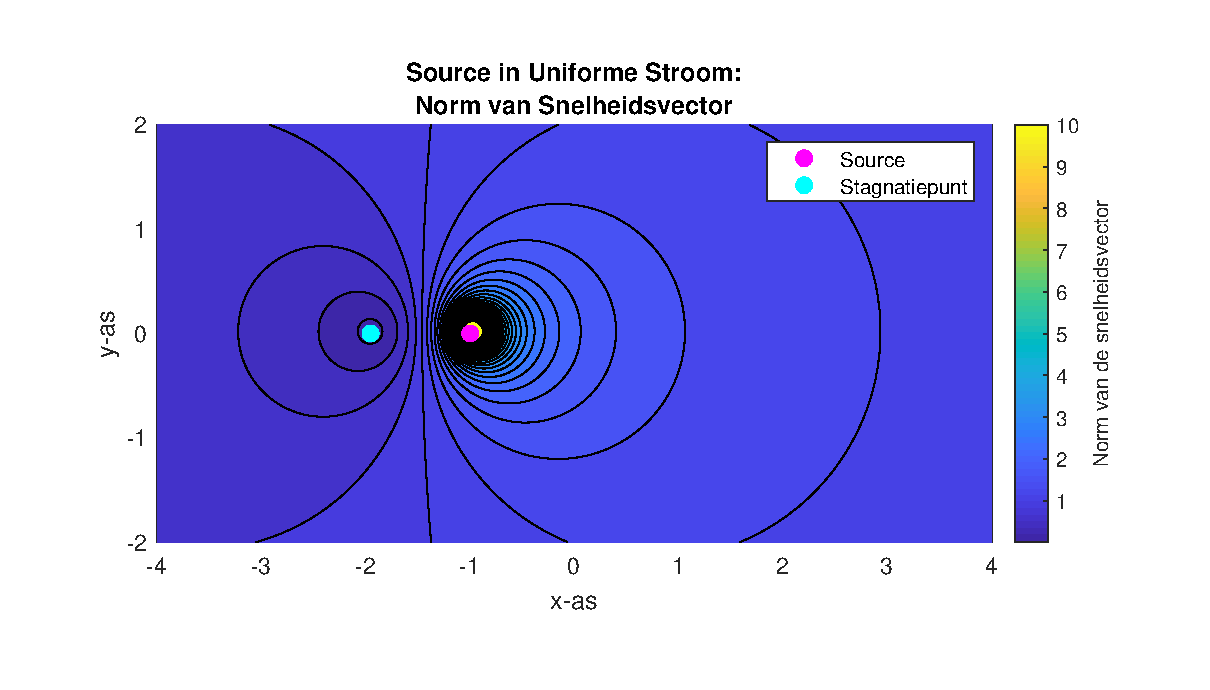
\includegraphics[width = \textwidth]{plots/probleem2_2.eps}
      \caption{Contourplot van de norm van de snelheidsvectoren.}
      \label{probleem2_2}
    \end{figure}
    \FloatBarrier

  \newpage
  \subsection{Probleem 3: Een source-sink pair in een uniform flow}
    \noindent
    Voor deze opdracht onderzoeken we een Rankine Oval, gevormd door een source-sink paar in een uniforme stroming. Voor een source-sink paar met gelijke sterkte in een uniforme stroom worden de stroomlijnen en snelheidsvectoren gevisualiseerd op figuur \ref{probleem3_1}. We kunnen eenvoudig bepalen welke stroomlijnen deze Rankine oval beschrijven, daar deze stroomlijnen ook door de stagnatiepunten lopen. We leiden de afmetingen van de Rankine oval af in functie van de sterkte van de source en sink. We beginnen hierbij vanuit de superpositie van stroomfuncties:\footnote{Gekende variabelen zoals positie en hoek zijn reeds ingevuld daar we de afmetingen slechts in functie van de sterktes willen bepalen.}

    \begin{equation*}
      \left\{
      \begin{align}
        \psi_{uniform}\p{x,y} &= U_\infty y \\
        \psi_{source}\p{x,y} &= \frac{Q}{2\pi}\arctan{\frac{y}{x+1}} \\
        \psi_{sink}\p{x,y} &= -\frac{Q}{2\pi}\arctan{\frac{y}{x-1}}
      \end{align}
      \right.
    \end{equation*}

    \noindent
    Waar direct uit volgt dat:

    \begin{equation*}
      \psi_{totaal}\p{x,y} =  U_\infty y+\frac{Q}{2\pi}\s{\arctan{\frac{y}{x+1}}-\arctan{\frac{y}{x-1}}}
    \end{equation*}

    \noindent
    Dan bepalen we de positie van de stagnatiepunten op analoge wijze aan de bepaling hiervan in opdracht 2, ook weten we uit de symmetrie van het probleem dat de stagnatiepunten gelegen zijn op $y = 0$, dus zullen we enkel zoeken waar $v_x$ nul wordt. We beginnen weer vanuit het superpositie beginsel:\footnote{Gekende variabelen zoals positie en hoek zijn reeds ingevuld.}

    \begin{equation*}
      \left\{
      \begin{align*}
        v_{uniform,x}\p{x,y} &= U_\infty \\
        v_{source,x}\p{x,y} &= \frac{Q}{2\pi}\frac{x+1}{(x+1)^2+y^2} \\
        v_{sink,x}\p{x,y} &= -\frac{Q}{2\pi}\frac{x-1}{(x-1)^2+y^2}
      \end{align*}
      \right.
    \end{equation*}

    \noindent
    Waar direct uit volgt dat:\footnote{Mits invullen van het gekende dat $y = 0$.}

    \begin{equation*}
      v_{totaal,x}\p{x,0} &= U_\infty + \frac{Q}{2\pi}\p{\frac{1}{x+1}-\frac{1}{x-1}}
    \end{equation*}

    \noindent
    Dit kunnen we dan oplossen naar $x$ door te stellen dat $v_{totaal}\p{x_{stagnatie},0} = 0$, dit levert na vereenvoudiging:

    \begin{equation*}
      x_{stagnatie} = \pm\sqrt{\frac{Q+\pi U_\infty}{\pi U_\infty}}
    \end{equation*}

    \noindent
    Dit komt dan ook overeen met de lengte van de halve lange as van de ellips beschreven door de Rankine oval. Om de korte lange as te bepalen van de ellips maken we gebruik van de stroomfunctie die we eerder hadden afgeleid en stellen dan dat de halve lange as gegeven wordt door $y$ waarvoor geldt dat:

    \begin{equation*}
      \psi\p{0,y} = \psi\p{x_{stagnatie},0}
    \end{equation*}

    \noindent
    Invullen geeft dan:

    \begin{align*}
      0 &= U_\infty y+\frac{Q}{2\pi}\s{\arctan{y}-\arctan{-y}} \\
      0 &= U_\infty y+\frac{Q}{\pi}\arctan{y}
    \end{align*}

    \noindent
    Dit geeft dan volgende relatie voor $y$, die enkel (numeriek) opgelost kan worden indien de sterktes ingegeven worden:

    \begin{equation*}
      y = \tan\p{\frac{\pi U_\infty y}{Q}}
    \end{equation*}

    \noindent
    Vervolgens werd ook de drukco\"effici\"ent berekend met de gegeven formule \cite{opdracht}, waarmee het contourplot op figuur \ref{probleem3_2} gevormd werd. Hierop zien we dat de drukco\"effic\"ent maximaal ($C_p = 1$) in de twee stagnatiepunten. Dit is een intu\"itief eenvoudig resultaat daar dit de enige twee punten zijn waarvan de stromen van de source/sink en de uniforme stroom ``botsen'' en tot een stilstand komen. \\

    \noindent
    Tot slot van deze opdracht keken we nog naar het geval waarbij de source en sink verschillende sterktes hebben, hiervoor is de weergave van de stroomlijnen en snelheidsvectoren gegeven op figuur \ref{probleem3_3}. Hierop hebben we de source sterker gemaakt dan de uniforme stroming en de sink, waarbij we een hybride figuur zien tussen de Rankine oval en Rankine half-body. Dit is enigzins logisch daar je dit systeem sou kunnen construeren door het optellen van 2 systemen:
    \begin{enumerate}
      \item Een systeem waar men de Rankine oval waarneemt.
      \item Een systeem waar men de Rankine half body waarneemt.
    \end{enumerate}

    \FloatBarrier
    \begin{figure}[ht!]
      \centering
      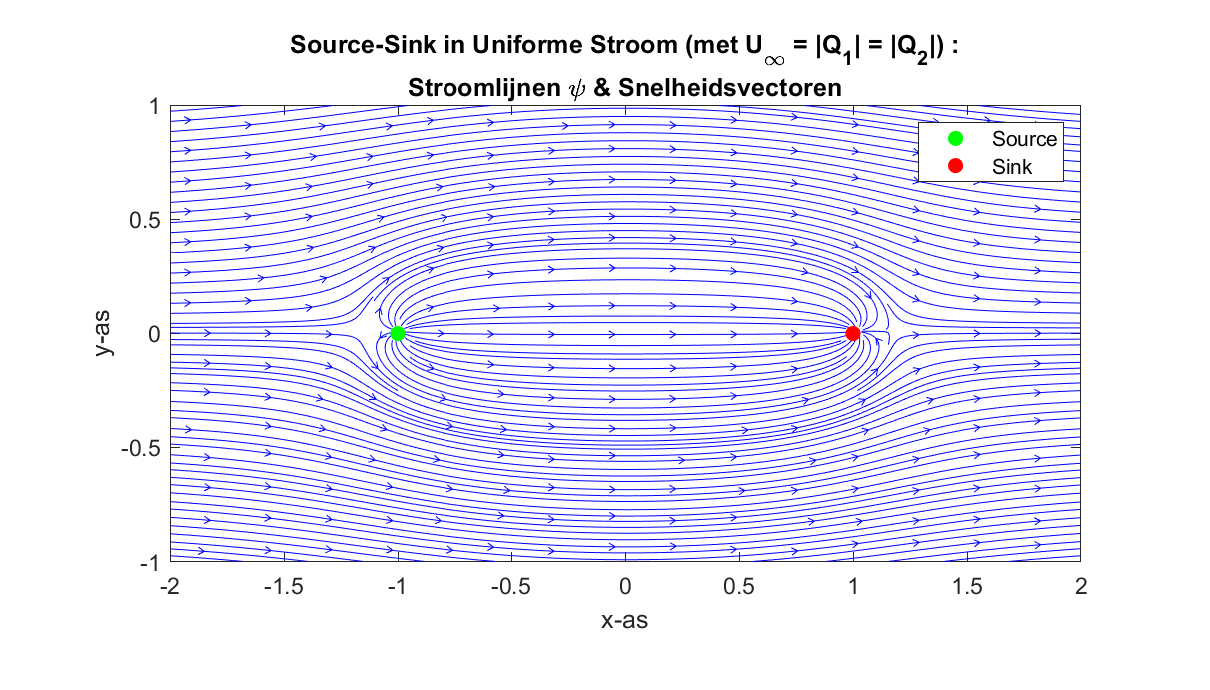
\includegraphics[width = \textwidth]{plots/probleem3_1.eps}
      \caption{Stroomlijnen en snelheidsvectoren van een source-sink paar in een uniforme stroom met gelijke sterkten ($Q_{source} = Q_{sink} = U_\infty$), met een duidelijke Rankine oval.}
      \label{probleem3_1}
    \end{figure}
    \begin{figure}[ht!]
      \centering
      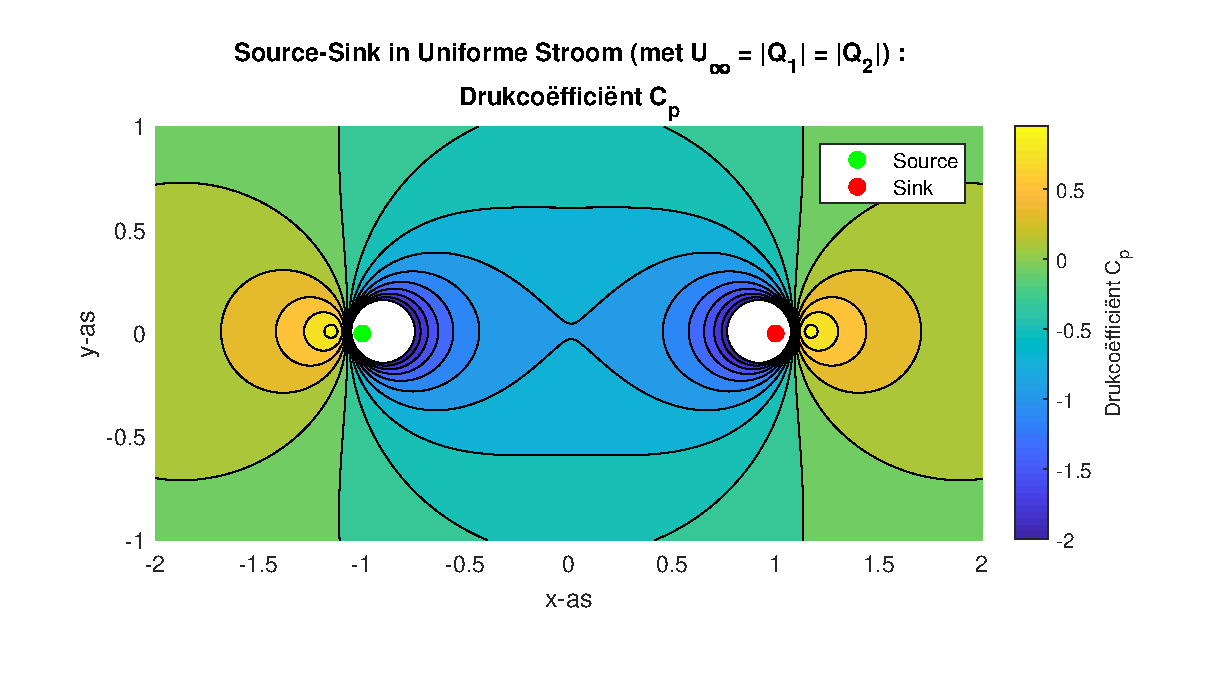
\includegraphics[width = \textwidth]{plots/probleem3_2.eps}
      \caption{Contourplot van de drukco\"effici\"ent $C_p$ voor een source-sink paar in uniforme stroom met gelijke sterkten. De twee stagnatiepunten zijn duidelijk zichtbaar daar de drukco\"effici\"ent $C_p$ maximaal wordt.}
      \label{probleem3_2}
    \end{figure}
    \begin{figure}[ht!]
      \centering
      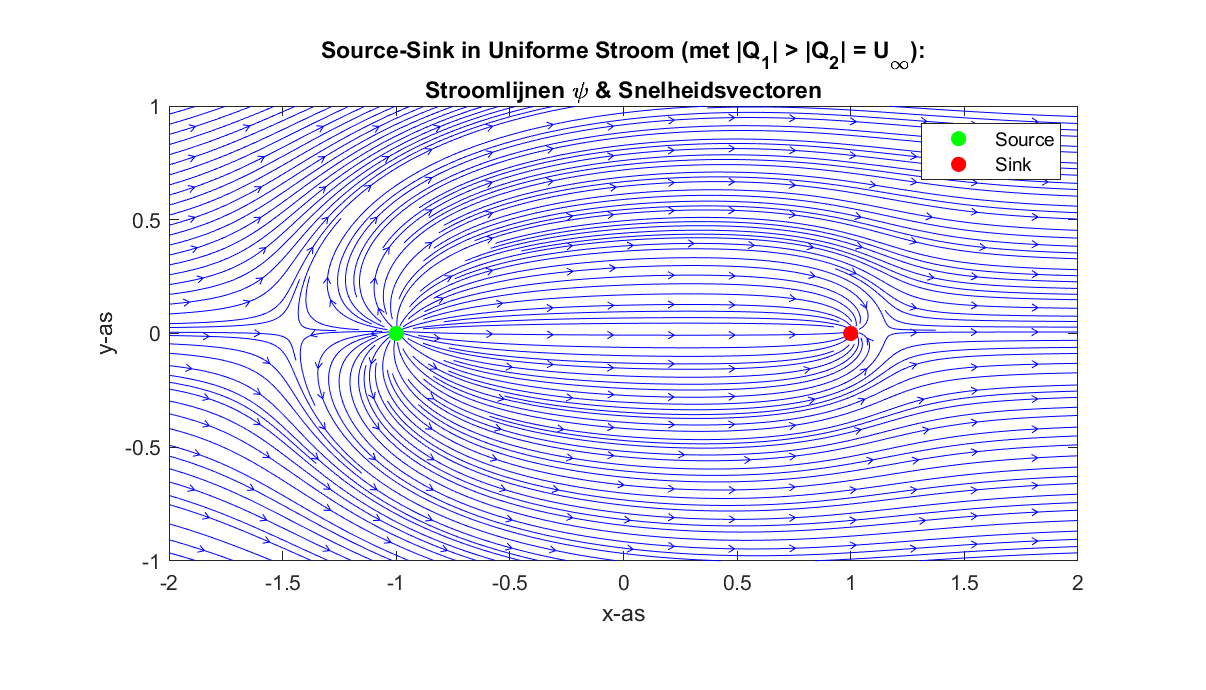
\includegraphics[width = \textwidth]{plots/probleem3_3.eps}
      \caption{Source-sink paar in een uniforme stroom met gelijke sterkten ($Q_{source} = Q_{sink} = U_\infty$), met een duidelijke Rankine oval.}
      \label{probleem3_3}
    \end{figure}
    \FloatBarrier



  \subsection{Probleem 4: Een source-sink doublet in een uniforme flow}
    \noindent
    In deze opdracht beschouwen we een source-sink doublet in een uniforme stroom. De snelheidsvectoren en stroomlijnen hiervoor zijn weergegeven in figuur \ref{probleem4_1}. We tonen dan dat de straal van de cirkel gegeven door de Rankin oval voor een doublet in uniforme stroming gegeven is door:

    \begin{equation*}
      a = \sqrt{\frac{\kappa}{2\pi U_\infty}}
    \end{equation*}

    \noindent
    Uit de literatuur \cite{cursus} weten we ook dat de Rankine oval gegeven wordt door de lijn daar de stroomfunctie $\psi$ gelijk is aan nul. We maken dan gebruik van het superpositiebeginsel om de stroomfunctie voor deze situatie opte stellen:

    \begin{equation*}
      \left\{
      \begin{align}
        \psi_{uniform}\p{x,y} &= U_\infty\p{y\cos\alpha+x\sin\alpha} \\
        \psi_{doublet}\p{x,y} &= -\frac{\kappa}{2\pi}\frac{y}{x^2+y^2}
      \end{align}
      \right.
    \end{equation*}

    \noindent
    Dit levert dan direct:\footnote{Na invullen van enkele gekende variabelen.}

    \begin{equation*}
      \psi_{totaal}\p{x,y} = U_\infty y - \frac{\kappa}{2\pi}\frac{y}{x^2+y^2}
    \end{equation*}

    \noindent
    We stellen deze dan $\psi_{totaal} = 0$ en herschikken de termen:

    \begin{equation*}
      x^2+y^2 = \frac{\kappa}{2\pi U_\infty}
    \end{equation*}

    \noindent
    Eenvoudige geometrie leert ons dat de straal $r$ gelijk is aan $x^2+y^2$ zodat er volgt dat de straal van de Rankine ovaal/cirkel hier gegeven is door:

    \begin{equation*}
      r = \sqrt{\frac{\kappa}{2\pi U_\infty}} \overset{!}{=} a
    \end{equation*}

    \noindent
    Vervolgens tonen we ook aan dat de drukco\"effici\"ent gegeven is door volgend voorschrift:\footnote{Op de cirkel met straal $a$.}

    \begin{equation*}
      C_p\p{r=a,\theta} = 1-4\sin^2\theta
    \end{equation*}

    \noindent
    We vertrekken hiervoor vanuit het gekende \cite{opdracht}:

    \begin{equation*}
      C_p\p{x,y} = 1-\frac{\s{V\p{x,y}}^2}{V_\infty^2}
    \end{equation*}

    \noindent
    Indien we dan ook de snelheid bepalen voor dit systeem in poolco\"ordinaten en ingeven dat $r = a$ kunnen we deze uitdrukking schrijven als:

    \begin{equation*}
      C_p\p{r,\theta} = 1-\frac{1}{U_\infty^2}\s{\p{U_\infty-\frac{\kappa}{2\pi}\frac{\cos^2\theta-\sin^2\theta}{a^2}}^2+\p{\frac{\kappa}{2\pi}\frac{2\cos\theta\sin\theta}{a^2}}^2}
    \end{equation*}

    \noindent
    Verder schrappen en verder uitwerken levert dan direct het gevraagde:

    \begin{equation*}
      C_p\p{r=a,\theta} \overset{!}{=} 1-4\sin^2\theta
    \end{equation*}

    \noindent
    Deze curve is geplot op figuur \ref{probleem4_2}. Wat hieraan opvalt is dat de drukco\"effici\"ent dus gelijk is op $\theta = 0$ en $\theta = \pi$; dit betekent dat in onsamendrukbare laminaire stroom er geen kracht uitgeoefend wordt op een cilinder in een uniforme stroom!
\newpage
    \FloatBarrier
    \begin{figure}[ht!]
      \centering
      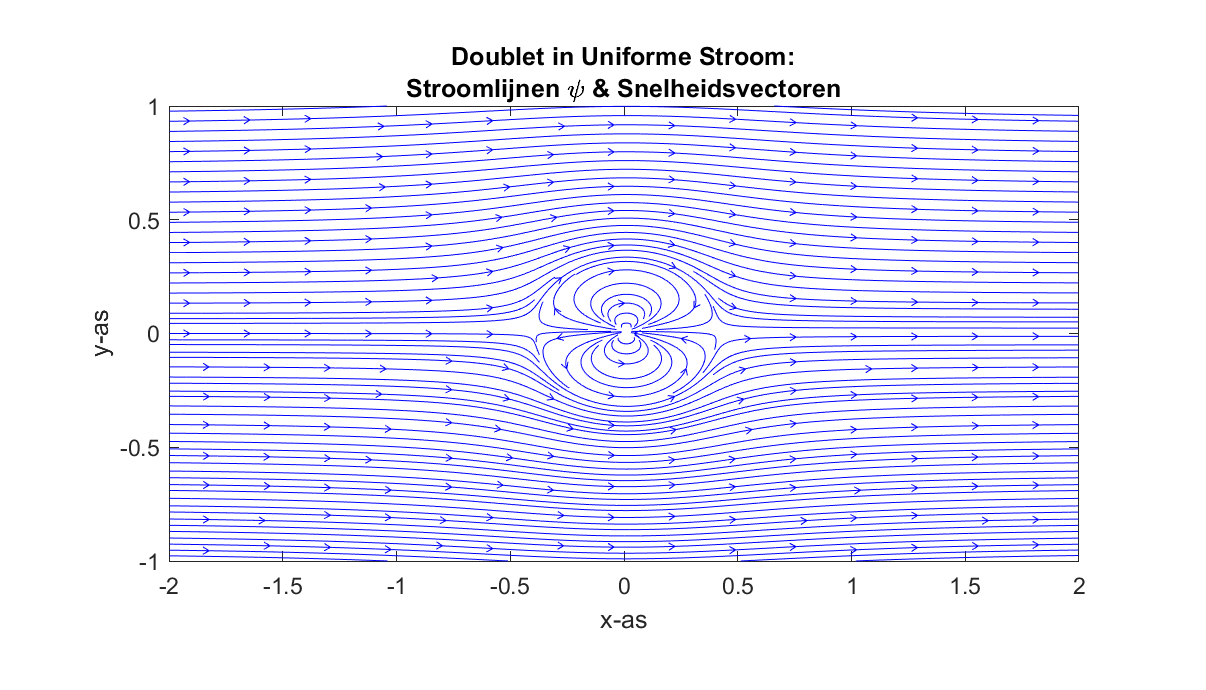
\includegraphics[width = \textwidth]{plots/probleem4_1.eps}
      \caption{Stroomlijnen en snelheidsvectoren voor een source-sink doublet in een uniforme stroming.}
      \label{probleem4_1}
    \end{figure}
    \begin{figure}[ht!]
      \centering
      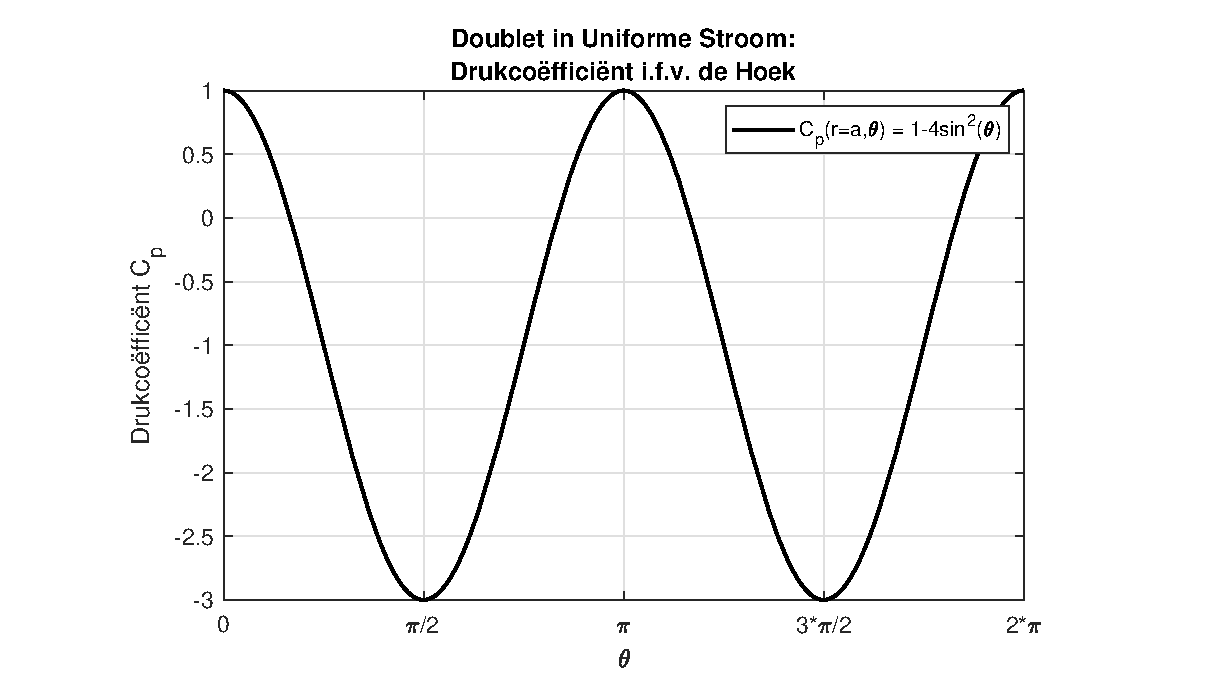
\includegraphics[width = \textwidth]{plots/probleem4_2.eps}
      \caption{Plot van de drukco\"effici\"ent op straal $a$ rond een doublet in uniforme stroom.}
      \label{probleem4_2}
    \end{figure}
    \FloatBarrier
\newpage
%\phantom{yeet}

\newpage
  \subsection{Probleem 5: Vortices}
    \noindent
    In deze opdracht onderzoeken we algemeen gebruik van vortices en de effecten van het combineren van verschillende vortices, wat we eerst numeriek aanpakken en dan met een analytische methode. Allereerst maken we een eenvoudige vortex in de oorsprong, waarvan de stroomlijnen en snelheidsvectoren weergegeven zijn op figuur \ref{probleem5_1}. We zien hier een typische cirkelvormige stroom die men zou verwachten van een vortex. Indien we deze vortex echter combineren met een sink (op dezelfde positie) zien we een heel intu\"itief resultaat opdagen, namelijk een waterkolk waarvan de stroomlijnen en snelheidsvectoren weergegeven zijn op figuur \ref{probleem5_2}.\\

    \noindent
    Dan kunnen we ook meerder vortices combineren en zo de effecten van een vortexsheet onderzoeken. Voor de numerieke methode zullen we $N$ vortices met gelijke sterkte plaatsen in het $x$ interval $[-2,2]$. Op figuur \ref{probleem5_3} geven we de stroomlijnen en snelheidsvectoren gevonden voor volgende waarden van $N$:

    \begin{equation*}
      N\in\left\{ 3, 4, 5, 10 \right\}
    \end{equation*}

    \noindent
    We zien dat de stromen boven en onder de vortices steeds evenwijdiger komen te liggen en in tegengestelde richting lopen. Dit zien we ook wanneer we de analytische oplossing voor een oneindige rij van vortices nemen zoals weergegeven op figuur \ref{probleem5_4}. We zien dus dat aangezien de stroom boven de vortices in de tegengestelde richting loopt aan de stroom onder de vortices kunnen we een vortexsheet (oneindig lang) gebruiken voor simulaties die werken aan het oppervlak tussen twee flu\"ida met verschillende snelheden.

    \FloatBarrier
    \begin{figure}[ht!]
      \centering
      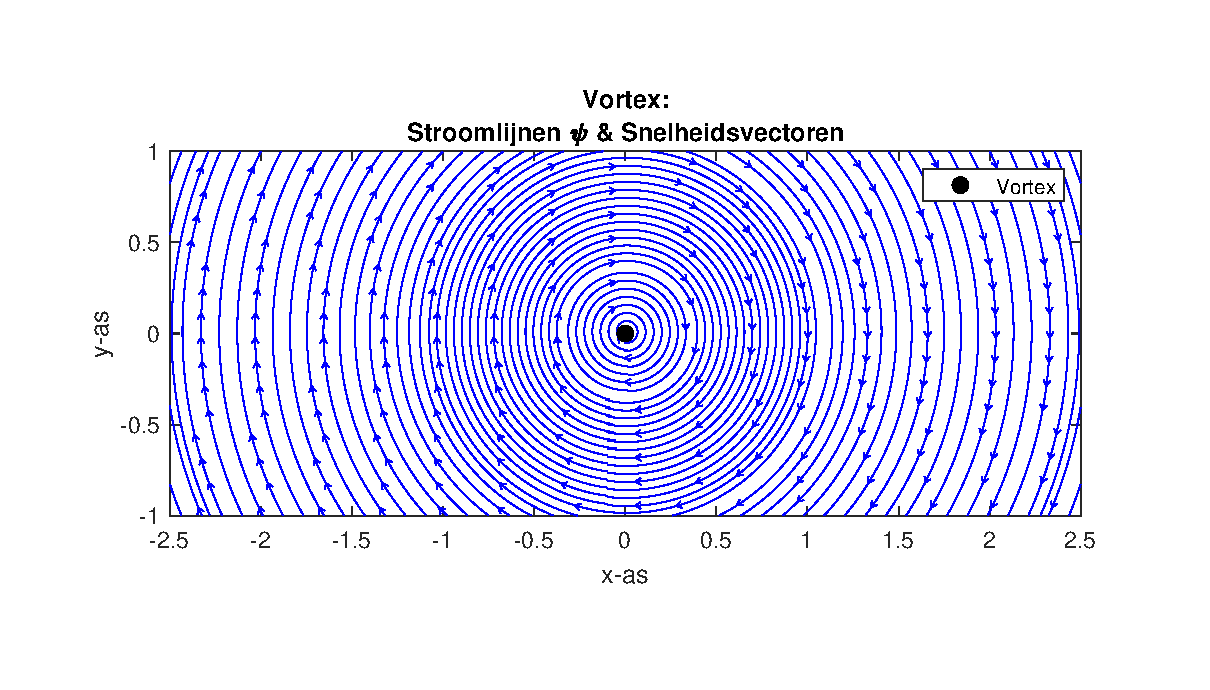
\includegraphics[width = \textwidth]{plots/probleem5_1.eps}
      \vspace{-1.5cm}\caption{Snelheidsvectoren en stroomlijnen van een vortex geven een cirkelvormige stroom.}
      \label{probleem5_1}
    \end{figure}
    \begin{figure}[ht!]
      \centering
      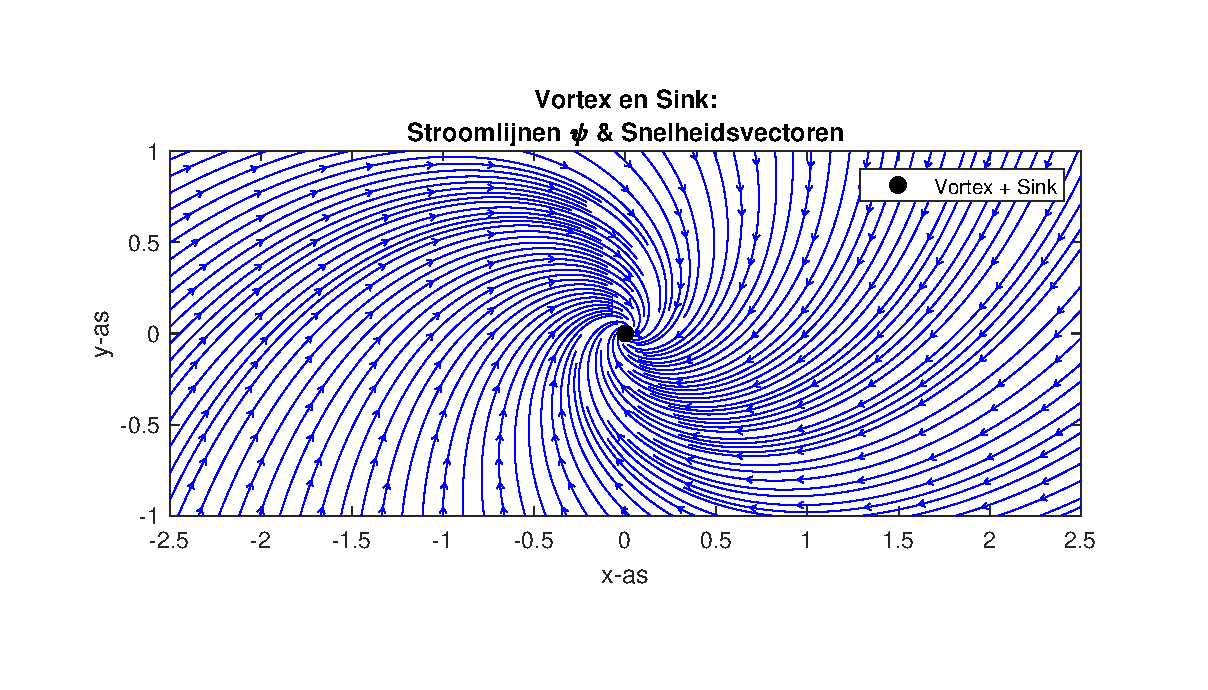
\includegraphics[width = \textwidth]{plots/probleem5_2.eps}
      \vspace{-1.5cm}\caption{Combinatie van een vortex met een sink geeft een draaikolk.}
      \label{probleem5_2}
    \end{figure}
    \begin{figure}[ht!]
      \centering\vspace{-1.5cm}
      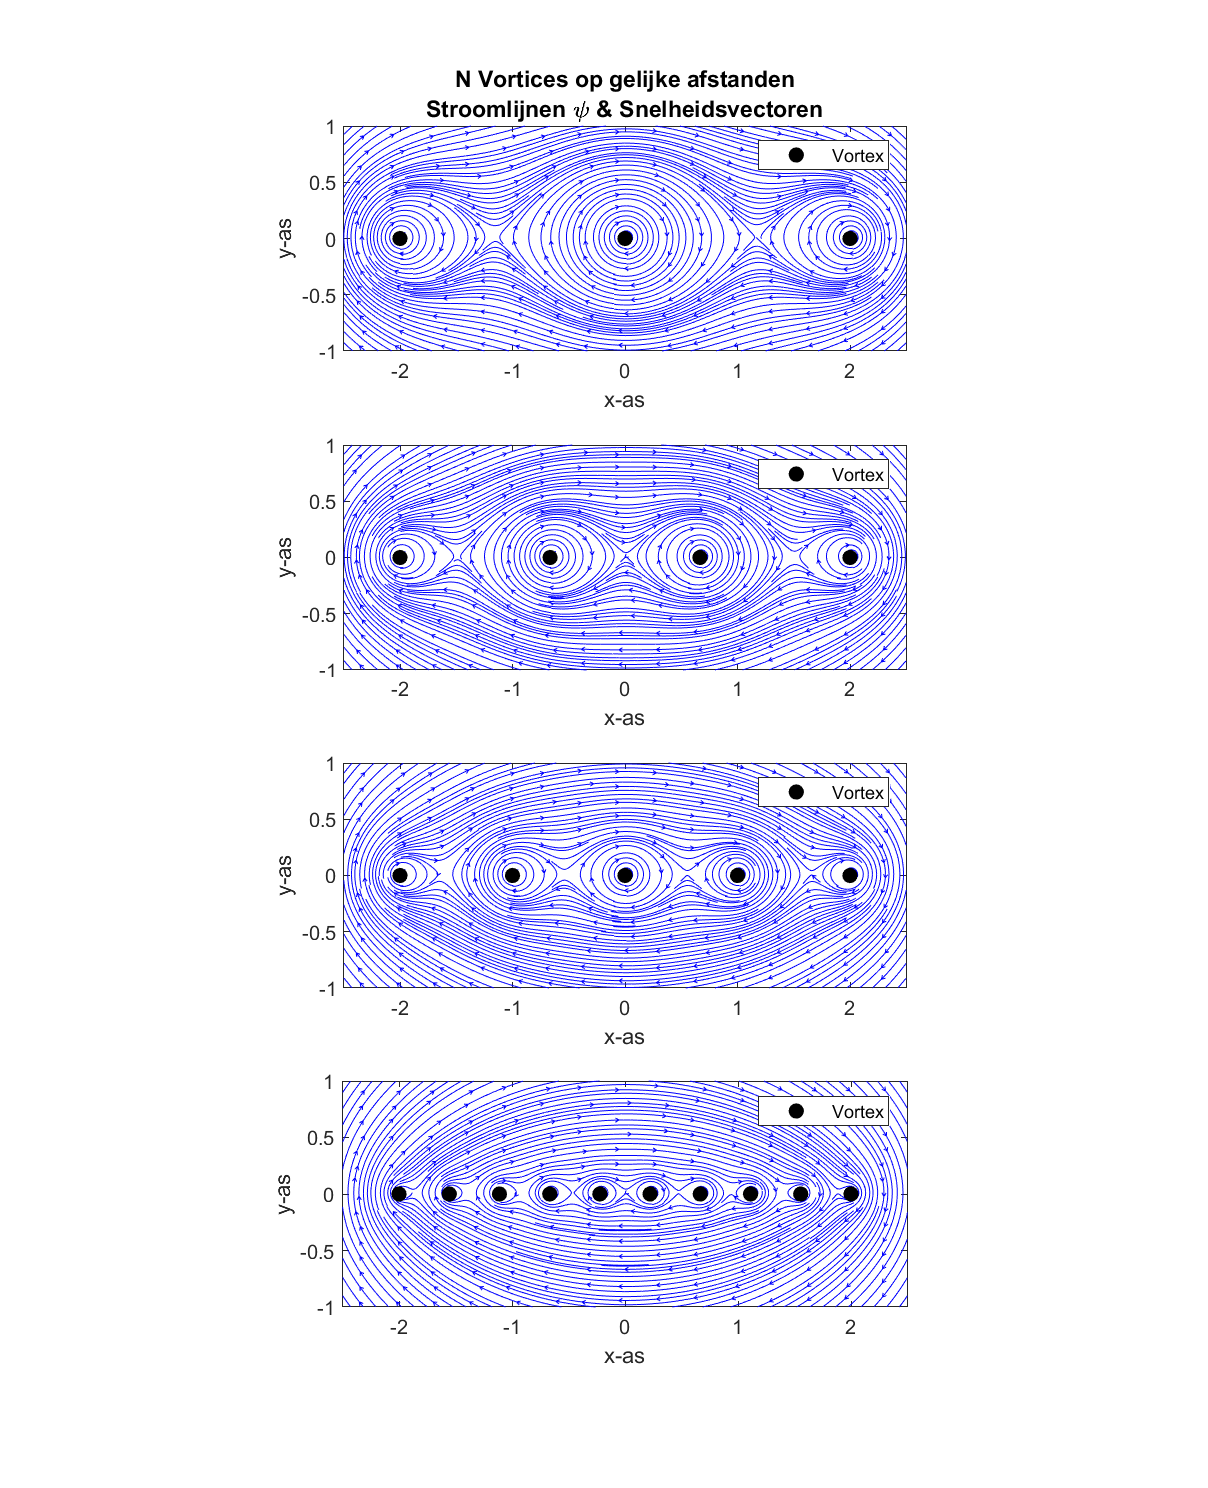
\includegraphics[width = \textwidth]{plots/probleem5_3.eps}\vspace{-1cm}
      \caption{De plots geven de stroomlijnen en snelheidsvectoren weer voor $N$ vortices equidistant geplaatst tussen $x\in[-2,2]$, voor $N\in\{ 3, 4, 5, 10 \}$.}
      \label{probleem5_3}
    \end{figure}
    \begin{figure}[ht!]
      \centering
      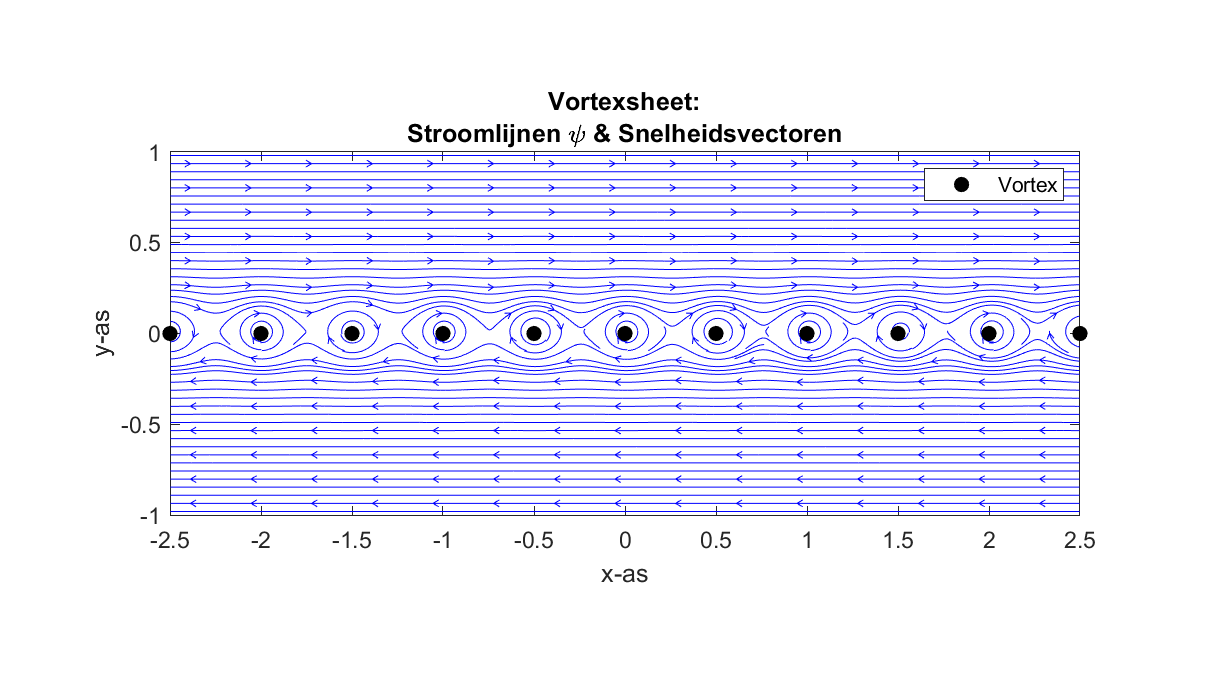
\includegraphics[width = \textwidth]{plots/probleem5_4.eps}
      \vspace{-1.5cm}\caption{Voor een oneindig lange reeks equidistante vortices vinden we dat de vortices een interface opleveren tussen twee stromen in tegengestelde richtingen.}
      \label{probleem5_4}
    \end{figure}
    \FloatBarrier
\newpage
  \subsection{Probleem 6: Lift op een vortex}
    \noindent
    In deze opdracht is gegeven dat (analoog aan opdracht 4) de straal van de Rankine oval/cirkel gegeven is door $R$ met:

    \begin{equation*}
      R = \sqrt{\frac{\kappa}{2\pi U_\infty}}
    \end{equation*}

    \noindent
    We zoeken dan de polaire hoek van de stagnatiepunten, hiervoor zullen we gebruik maken van superpositiebeginselen voor de snelheidsvectoren. Voor de $x$-component van de snelheidsvector vinden we:

    \begin{equation*}
      \left\{
      \begin{align}
        v_{vortex,x}\p{x,y} &= \frac{\Gamma}{2\pi}\frac{y}{x^2+y^2} \\
        v_{doublet,x}\p{x,y} &= -\frac{\kappa}{2\pi}\frac{x^2-y^2}{x^2+y^2} \\
        v_{uniform,x}\p{x,y} &= U_\infty\cos\alpha
      \end{align}
      \right.
    \end{equation*}

    \noindent
    Na optellen en invullen dat $\alpha = 0$ volgt er dat:

    \begin{equation*}
      v_{totaal,x}\p{x,y} = \frac{\Gamma}{2\pi}\frac{y}{x^2+y^2}-\frac{\kappa}{2\pi}\frac{x^2-y^2}{x^2+y^2}+U_\infty
    \end{equation*}

    \noindent
    We doen hetzelfde voor de $y$-component van de snelheid:

    \begin{equation*}
      \left\{
      \begin{align}
        v_{vortex,y}\p{x,y} &= -\frac{\Gamma}{2\pi}\frac{x}{x^2+y^2} \\
        v_{doublet,y}\p{x,y} &= -\frac{\kappa}{2\pi}\frac{2xy}{x^2+y^2} \\
        v_{uniform,y}\p{x,y} &= U_\infty\sin\alpha
      \end{align}
      \right.
    \end{equation*}

    \noindent
    Zodat na optellen en stellen dat $\alpha = 0$ volgt dat:

    \begin{equation*}
      v_{totaal,y} = -\frac{\Gamma}{2\pi}\frac{x}{x^2+y^2}-\frac{\kappa}{2\pi}\frac{2xy}{x^2+y^2}
    \end{equation*}

    \noindent
    Nu kunnen we met deze twee uitdrukkingen voor de componenten van de snelheid de stagnatiepunten bepalen, allereerst stellen we $v_y\p{x_{stagnatie},y_{stagnatie}} = 0$ en maken we gebruik van $x^2 + y^2 = R^2 = \frac{\kappa}{2\pi U_\infty}$, herschikken opdat we een oplossing voor $y_{stagnatie}$ vinden levert dan direct dat:

    \begin{equation*}
      y_{stagnatie} = -\frac{\Gamma}{4\pi U_\infty}
    \end{equation*}

    \noindent
    Nu deze gekend is kunnen we op analoge wijze de $x$ positie van de stagnatiepunten bepalen door middel van het stellen dat $v_x\p{x_{stagnatie},y_{stagnatie}} = 0$ en weer gebruik te maken van $x^2+y^2 = R^2$, dit levert dan na oplossen naar $x_{stagnatie}$ en vereenvoudiging dat:

    \begin{equation*}
      x_{stagnatie} = \pm\sqrt{\frac{2\pi}{\kappa U_\infty}}\p{U_\infty-\frac{\Gamma^2}{4\pi\kappa}}
    \end{equation*}

    \noindent
    We kunnen dan eenvoudig de polaire hoek $\theta_{stagnatie}$ bepalen:

    \begin{equation*}
      \theta_{stagnatie} = \arctan{\frac{y_{stagnatie}}{x_{stagnatie}}} = \arctan{\frac{\mp\Gamma}{4\piU_\infty\sqrt{\frac{2\pi}{\kappa U_\infty}}\p{U_\infty-\frac{\Gamma^2}{4\pi\kappa}}}}
    \end{equation*}

    \noindent
    Merk dan ook op dat wanneer er niet voldaan is aan volgend criterium, er geen oplossing bestaat voor $\theta_{stagnatie}$:

    \begin{equation*}
      \frac{\Gamma}{4\pi U_\infty R} > 1
    \end{equation*}

    \noindent
    Een geval hiervan is gevisualiseerd op figuur \ref{probleem6_2}. We zien hierop dat de vortex een overheersend effect zal krijgen; er is enkel een assymmetrische vortex zichtbaar op de figuur. \\

    \noindent
    Dan kunnen we nog tot slot van deze opdracht de drukco\"effici\"enten (op het oppervlak van de Rankine oval/cirkel, dus $r = R$) bepalen voor volgende twee configuraties:
    \begin{enumerate}
      \item Doublet in uniforme stroom.
      \item Doublet + vortex in uniforme stroom.
    \end{enumerate}

    \noindent
    Eerst bepalen we die voor het doublet in uniforme stroom, we maken gebruik van de uitdrukkingen voor snelheden in poolco\"ordinaten:\footnote{We maken gebruik van de gegeven uitdrukkingen voor de stroomfuncties in poolco\"ordinaten en dan maken we gebruik van de gegeven relaties tussen snelheidsvectoren en stroomfuncties \cite{opdracht}.}$^{,}$\footnote{We geven reeds in dat $\alpha = 0$.}

    \begin{equation*}
      \left\{
      \begin{align}
        v_{uniform,r}\p{r,\theta} &= U_\infty\cos\theta \\
        v_{uniform,\theta}\p{r,\theta} &= -U_\infty\sin\theta \\
        v_{doublet,r}\p{r,\theta} &= -\frac{\kappa}{2\pi}\frac{\cos\theta}{r^2} \\
        v_{doublet,\theta}\p{r,\theta} &= \frac{\kappa}{2\pi}\frac{\sin\theta}{r^2}
      \end{align}
      \right.
    \end{equation*}

    \noindent
    Dan is de drukco\"effici\"ent gegeven door:

    \begin{align*}
      C_p\p{r = R,\theta} &= 1-\frac{v_{totaal,r}^2+v_{totaal,\theta}^2}{U_\infty^2} \\
      &= ...
    \end{align*}

    \noindent
    ////UITLEG

    \begin{equation*}
      \left\{
      \begin{align}
        v_{vortex,r}\p{r,\theta} &= 0 \\
        v_{vortex,\theta}\p{r,\theta} &= \frac{\Gamma}{2\pi r}
      \end{align}
      \right.
    \end{equation*}

    \noindent
    Zodat:

    \begin{align*}
      C_p\p{r = R,\theta} &= ...
    \end{align*}

    \FloatBarrier
    \begin{figure}[ht!]
      \centering
      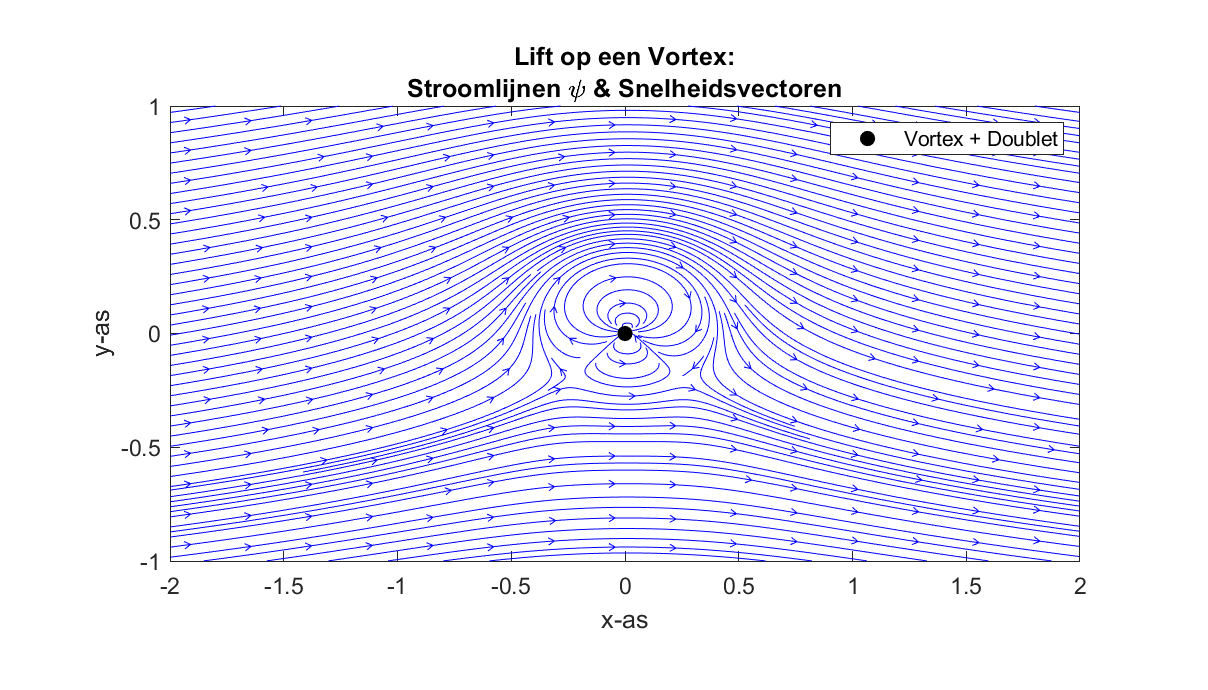
\includegraphics[width = \textwidth]{plots/probleem6_1.eps}
      \caption{Snelheidsvectoren en stroomlijnen voor een systeem met vortex en doublet in de oorspronk in een uniforme stroom.}
      \label{probleem6_1}
    \end{figure}
    \begin{figure}[ht!]
      \centering
      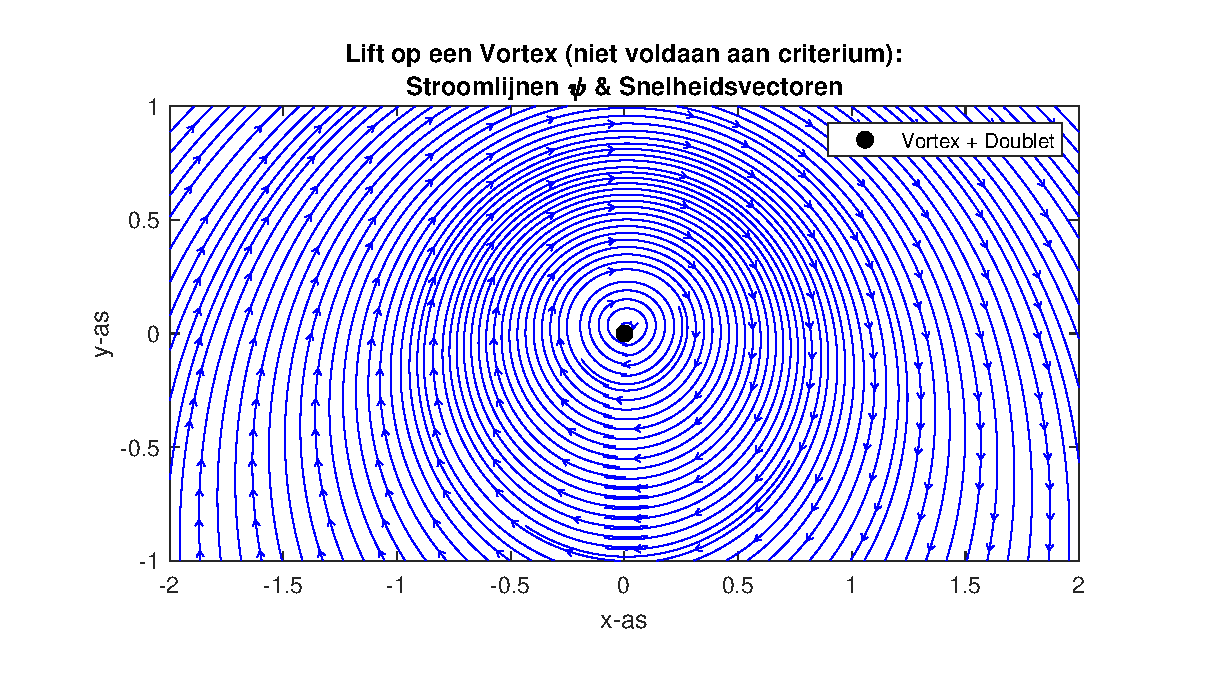
\includegraphics[width = \textwidth]{plots/probleem6_2.eps}
      \caption{Snelheidsvectoren en stroomlijnen voor een systeem als in figuur \ref{probleem6_1}, maar dat niet voldoet aan het criterium.}
      \label{probleem6_2}
    \end{figure}
    \begin{figure}[ht!]
      \includegraphics[width = \textwidth]{plots/probleem6_3.eps}
      \caption{Drukco\"effici\"ent in functie van de polaire hoek voor een doublet in uniforme stroom.}
      \label{probleem6_3}
    \end{figure}
    \begin{figure}[ht!]
      \includegraphics[width = \textwidth]{plots/probleem6_4.eps}
      \caption{Drukco\"effic\"ent in functie van de polaire hoek voor een doublet en vortex in uniforme stroom.}
      \label{probleem6_4}
    \end{figure}
    \FloatBarrier



\section{Conclusie}

\newpage
\begin{thebibliography}{99}
  \bibitem{opdracht} N. van Remortel \& M. Verstraeten (2019). \textit{Examenopdracht Inleiding Programmeren: Numerieke benadering van aerodynamische problemen met behulp van potentiaalstromings theorie}, UAntwerpen.
  \bibitem{cursus} C. Beaume (ONGEKEND). \textit{Fundamentals of Fluid Mechanics}, Department of Aeronautics // Imperial College London.
\end{thebibliography}

\end{document}
